\documentclass[11pt,a4paper]{amsart}
\usepackage[utf8]{inputenc}
\usepackage[T1]{fontenc}
\usepackage{lmodern}
\usepackage{amsmath,amssymb,amsthm}
\usepackage{booktabs}
\usepackage{graphicx}
\usepackage[margin=2.0cm]{geometry}
\usepackage{xcolor}
\usepackage[colorlinks=true,linkcolor=blue!50!black,citecolor=blue!50!black,urlcolor=blue!50!black]{hyperref}

\newtheorem{theorem}{Theorem}
\newtheorem{lemma}[theorem]{Lemma}
\newtheorem{proposition}[theorem]{Proposition}
\newtheorem{corollary}[theorem]{Corollary}
\newtheorem*{thmA}{Theorem 3.2 of \cite{AN}}
\newtheorem*{thmB}{Theorem 4.8 of \cite{AN}}
\newtheorem*{thmAc}{Theorem 3.2$'$ (corrected)}
\newtheorem*{thmBc}{Theorem 4.8$'$ (corrected)}
\theoremstyle{remark}
\newtheorem{remark}[theorem]{Remark}
\newtheorem{example}[theorem]{Example}

\newcommand{\F}{\mathbb{F}}
\newcommand{\Fq}{\mathbb{F}_q}
\newcommand{\Fqn}{\mathbb{F}_{q^n}}
\newcommand{\Tr}{\mathrm{Tr}}
\newcommand{\Ord}{\mathrm{Ord}}

\title[Pairs of $r$-primitive and $k$-normal elements]{A note on the existence of pairs of $r$-primitive and $k$-normal elements over finite fields}
\author{Ruqing Chen}
\address{GUT Geoservice Inc., Montreal, Canada}
\email{ruqing@hotmail.com}
\date{November 2026}
\thanks{DOI: \href{https://doi.org/10.5281/zenodo.24313540}{10.5281/zenodo.24313540}. Code and data:
\href{https://github.com/Ruqing1963/aguirre-neumann-2022-pairs-audit}{github.com/Ruqing1963/aguirre-neumann-2022-pairs-audit}.}
\subjclass[2020]{12E20, 11T23}
\keywords{$r$-primitive elements, $k$-normal elements, rational functions, character sums, sieve}

\begin{document}
\begin{abstract}
We revisit J.~J.~R.~Aguirre and V.~G.~L.~Neumann, \emph{Pairs of $r$-primitive and $k$-normal elements in finite
fields} (arXiv:2210.11504; Bull.\ Braz.\ Math.\ Soc.\ 2023). Its Theorem~3.2 gives an inequality which, for every
rational function $F$ in a class $\Upsilon_{q^n}(m_1,m_2)$, is said to guarantee an $r_1$-primitive $k_1$-normal $\alpha$
with $F(\alpha)$ $r_2$-primitive $k_2$-normal. The class contains $F=x+1$. For $q=2$, $n=19$, $r_i=1$, $k_i=0$ the
inequality holds ($2^{9.5}\approx724\ge128$), but $\Tr(\alpha+1)=\Tr(\alpha)+1$, so $\alpha$ and $\alpha+1$ are never
both normal. The same happens for $F=x^2+x$. The proof leaves out the terms with $\eta_2$ trivial and $\psi_2$
nontrivial. For affine $F$ these terms have size $q^n$, not $O(q^{n/2})$. The summary Theorem~4.8 fails in the same
way: if $p\mid n$ or $\gcd(n,q-1)=1$, no affine $F=ax+b$ maps a $2$-normal element to a $1$-normal one. At $(q,n)=(5,10)$
an exhaustive search finds that the $16$ affine members of $\Upsilon_5(2,1)$ give no pair, while each of the other $560$
gives at least $3800$. We state the corrected theorems. We also point out an independent numerical gap: the
procedure TotalSieve prints the constant $6$ where the sieve criterion needs $36$. Of the $709$ pairs $(q,n)$ with
$q\le400$, $8\le n\le20$ covered by Theorem~4.8, $202$ cannot be certified by the sieve, $144$ of them even with
the constant $6$.
\end{abstract}
\maketitle

\section{Setting and statements}

Let $\Fqn\supset\Fq$ have characteristic $p$. An element is \emph{$r$-primitive} if its multiplicative order is
$(q^n-1)/r$, and \emph{$k$-normal} if its $\Fq$-order $\Ord(\alpha)$ (the monic generator of
$\{h\in\Fq[x]:h\circ\alpha=0\}$, where $h\circ\alpha=\sum h_i\alpha^{q^i}$) has degree $n-k$ \cite{HMPT}. Line numbers
``l.'' refer to the \LaTeX{} source of arXiv:2210.11504\,v1 \cite{AN}. A journal version appeared as
\cite{ANjournal}; we have only checked the arXiv text. Definition~2.1 (l.\,159--167) reads:
\begin{quote}\small
$\Upsilon_q(m_1,m_2)$ is the set of $F_1/F_2\in\Fq(x)$ such that (1) $\deg F_1\le m_1$, $\deg F_2\le m_2$;
(2) $\gcd(F_1,F_2)=1$; (3) there exist $m\in\mathbb{N}$ and an irreducible monic $g\in\Fq[x]\setminus\{x\}$ such that
$\gcd(m,q-1)=1$, $g^m\mid F_1F_2$ and $g^{m+1}\nmid F_1F_2$.
\end{quote}
Section~3 uses $\Upsilon_{q^n}(m_1,m_2)$, that is, coefficients in $\Fqn$ and $\gcd(m,q^n-1)=1$. Every $F=ax+b$ with
$a,b\neq0$ belongs to it: take $g=x+b/a$ and $m=1$.

\begin{thmA}[l.\,653--673]
Let $M=\max\{2(m_1+m_2),m_1+3m_2+1\}$, $1\le m_1+m_2<q^{n/2}$, $F\in\Upsilon_{q^n}(m_1,m_2)$, and let $f_i\mid x^n-1$
have degree $k_i$. If
\begin{equation}\label{eq:thm32}
q^{\frac n2-k_1-k_2}\ \ge\ M r_1r_2\,W\!\Big(\frac{q^n-1}{r_1}\Big)W\!\Big(\frac{q^n-1}{r_2}\Big)
W\!\Big(\frac{x^n-1}{f_1}\Big)W\!\Big(\frac{x^n-1}{f_2}\Big),
\end{equation}
then there is an $r_1$-primitive $k_1$-normal $\alpha\in\Fqn$ with $F(\alpha)$ $r_2$-primitive $k_2$-normal.
\end{thmA}

\begin{thmB}[l.\,1978--1989]
Let $F\in\Upsilon_q(2,1)$. If $n\ge8$, there is a $2$-primitive $2$-normal $\alpha\in\Fqn$ with $F(\alpha)$
$3$-primitive $1$-normal if and only if $6\mid q^n-1$ and $\gcd(q^3-q,n)\ne1$. For $n=7$ and $q\ge5.259\cdot10^{15}$
the same holds with the condition $6\mid q-1$ and $7\mid q^3-q$.
\end{thmB}

\section{Counterexamples}\label{sec:ce}

\begin{example}[Theorem~3.2, $q=2$, $n=19$]\label{ex:219}
Take $r_1=r_2=1$, $k_1=k_2=0$ (so $f_1=f_2=1$) and $F=x+1\in\Upsilon_{2^{19}}(1,0)$, so $M=2$. Here $2^{19}-1=524287$
is prime, so $W(2^{19}-1)=2$. The order of $2$ modulo $19$ is $18$, so $x^{19}-1=(x+1)\Phi_{19}(x)$ with $\Phi_{19}$
irreducible over $\F_2$, and $W(x^{19}-1)=4$. The right side of \eqref{eq:thm32} is $2\cdot2\cdot2\cdot4\cdot4=128$,
and the left side is $2^{9.5}\approx724.1$. The theorem therefore asserts a primitive normal $\alpha$ with $\alpha+1$
primitive normal. However, $\Tr(\beta)=T\circ\beta$ with $T=(x^{19}-1)/(x+1)$, so a normal element of $\F_{2^{19}}$
has trace $1$. Since $\Tr(\alpha+1)=\Tr(\alpha)+19=\Tr(\alpha)+1$, at most one of $\alpha$, $\alpha+1$ is normal.
An exhaustive enumeration of $\F_{2^{19}}$ confirms this. There are $262143$ normal elements, all primitive and all of
trace $1$, and no $\alpha$ has both $\alpha$ and $\alpha+1$ normal.

The phenomenon is not tied to degree~$1$. The polynomial $F=x^2+x=x(x+1)$ lies in $\Upsilon_{2^{19}}(2,0)$ (take
$g=x+1$), so $M=4$, and the right side of \eqref{eq:thm32} is $256\le724.1$. But $\Tr(\alpha^2+\alpha)=0$ for every
$\alpha$, so $F(\alpha)$ is never normal. The enumeration again finds no pair.
\end{example}

For Theorem~4.8 the obstruction comes from the module structure, not from the trace.

\begin{lemma}\label{lem:affine}
Let $a,b\in\Fq^*$ and $\alpha\in\Fqn$. Write $x^n-1=(x-1)^{N}G$ with $(x-1)\nmid G$, and let $c(\alpha)$ be the
exponent of $x-1$ in $\Ord(\alpha)$. Then $\Ord(a\alpha+b)$ and $\Ord(\alpha)$ have the same $G$-part, and if
$c(\alpha)\ge2$ then $\Ord(a\alpha+b)=\Ord(\alpha)$.
\end{lemma}
\begin{proof}
Multiplication by $a\in\Fq^*$ commutes with $h\circ$, so $\Ord(a\alpha)=\Ord(\alpha)$. Write
$\Fqn=V_1\oplus V_G$ with $V_1=\ker(x-1)^N$ and $V_G=\ker G$. Then $V_1$ is cyclic, $V_1\cong\Fq[x]/((x-1)^N)$, since
$\Fqn$ is a cyclic $\Fq[x]$-module. The constant $b$ lies in $\ker(x-1)\subset V_1$, so adding $b$ changes only the
$V_1$-component $\beta$ of $a\alpha$. In a cyclic module the kernels $\ker(x-1)^j$ form a chain, and
$\ker(x-1)\subseteq\ker(x-1)^{c-1}$ for $c\ge2$. So $\beta$ and $\beta+b$ have the same exponent $c$.
\end{proof}

\begin{proposition}\label{prop:affine}
Let $p\ge5$ and $a,b\in\Fq^*$. Suppose that $p\mid n$, or that $p\nmid n$ and $\gcd(n,q-1)=1$. Then $a\alpha+b$ is
not $1$-normal for any $2$-normal $\alpha\in\Fqn$. Hence the ``if'' part of Theorem~4.8 fails for $F=ax+b$ at every
such $(q,n)$ in its range.
\end{proposition}
\begin{proof}
If $p\mid n$, then $N=p^e\ge5$. A $2$-normal $\alpha$ has $\deg\Ord(\alpha)=n-2$, so $c(\alpha)\ge N-2\ge3$, and
$a\alpha+b$ is again $2$-normal by Lemma~\ref{lem:affine}. If $p\nmid n$ and $\gcd(n,q-1)=1$, then $N=1$ and $x-1$ is
the only linear factor of $x^n-1$. The degree-$2$ divisor $(x^n-1)/\Ord(\alpha)$ is squarefree and has at most one
linear factor, so it is an irreducible quadratic. Hence $c(\alpha)=1$. Adding $b$ can only change $c$ to $0$ or leave
it at $1$, so $\deg\Ord(a\alpha+b)\in\{n-3,n-2\}$.
\end{proof}

Both cases occur in the range of Theorem~4.8. If $p\mid n$, then $p\mid\gcd(q^3-q,n)$; examples are $(5,10)$,
$(7,14)$, $(5,20)$, and every $(q,n)$ with $p\ge5$ and $2p\mid n$. Examples of the second case are $(13,35)$ and
$(19,25)$. For $n=7$, every $q\equiv1\pmod 6$ with $q\equiv0$ or $-1\pmod 7$ is a counterexample.

\begin{example}[$(q,n)=(5,10)$, exhaustive]\label{ex:510}
Over $\F_5$, $x^{10}-1=(x-1)^5(x+1)^5$. We enumerated all of $\F_{5^{10}}$ and computed $\Ord(\alpha)$ from the
primary decomposition. We cross-checked $\deg\Ord$ against the rank of $(\alpha,\alpha^q,\dots,\alpha^{q^{n-1}})$ on
a random sample. There are $111280$ elements that are $2$-primitive and $2$-normal, and $371320$ that are $3$-primitive
and $1$-normal. Up to scaling of $F_2$, $\Upsilon_5(2,1)$ has $576$ members, $16$ of them affine ($ax+b$,
$a,b\in\F_5^*$). For each affine $F$, all $111280$ images $F(\alpha)$ are $2$-normal, as
Proposition~\ref{prop:affine} predicts, so there is no pair. Each of the other $560$ members has between $3800$ and
$4780$ admissible $\alpha$ (Figure~\ref{fig}(a)). Thus the obstruction of Proposition~\ref{prop:affine} is the only one at $(5,10)$: every affine $F$ fails and every non-affine $F$ succeeds. Since $(5,10)$ satisfies $6\mid5^{10}-1$ and
$\gcd(120,10)=10$, Theorem~4.8 (and Proposition~4.4(a), which covers $n=10$) is false here.
\end{example}

\begin{figure}[t]
\centering
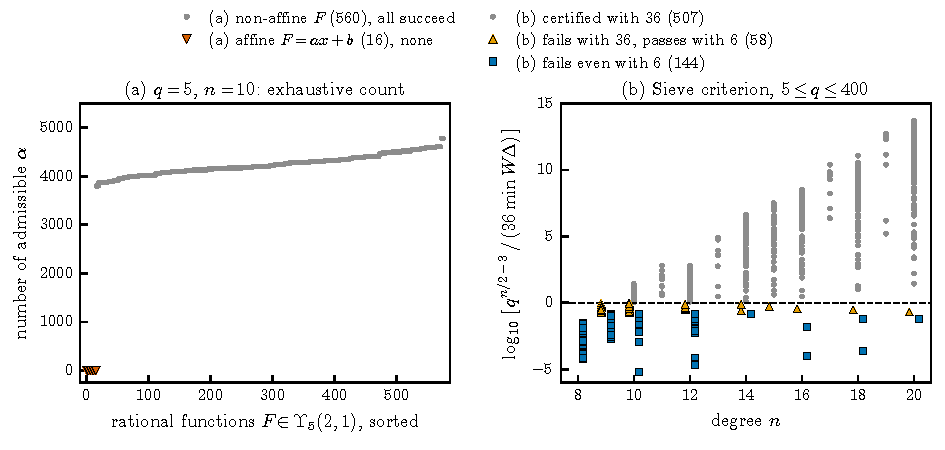
\includegraphics[width=0.84\textwidth]{figures/fig_aguirre_neumann_2022_audit.pdf}
\caption{(a) Exhaustive count at $(q,n)=(5,10)$. For each $F\in\Upsilon_5(2,1)$ (sorted by the count), the number of
$2$-primitive $2$-normal $\alpha$ with $F(\alpha)$ $3$-primitive $1$-normal. The $16$ affine $F$ have none; the others
have between $3800$ and $4780$. (b) The margin $\log_{10}$ of $q^{n/2-3}/(36\min W\Delta)$ in criterion~(3) for the
$709$ pairs $(q,n)$, $5\le q\le400$, $8\le n\le20$, in the range of Theorem~4.8 (markers offset slightly by class).
Points below the dashed line are not certified by any choice in Proposition~3.4.}\label{fig}
\end{figure}

\section{Where the proof fails}\label{sec:proof}

After Lemma~2.8, the proof of Theorem~3.2 reduces everything to (l.\,732--735)
\[
S(\eta_{d_1},\eta_{d_2},\psi_1,\psi_2)=\sum_{\alpha\in\Fqn^*\setminus S_F}\eta_{d_1}(\alpha)\eta_{d_2}(F(\alpha))
\psi_1(\alpha)\psi_2(F(\alpha))
\]
and claims $|S|\le Mq^{n/2}$ except when all four characters are
trivial (l.\,897--900). It announces ``six cases'' (l.\,739):
(i) all four trivial; (ii) $\eta_{d_2},\psi_2$ trivial, $\psi_1$ nontrivial; (iii) only $\eta_{d_1}$ nontrivial;
(iv) $\eta_{d_2}$ nontrivial, $\psi_1,\psi_2$ trivial; (v) $\eta_{d_2}$, $\psi_1$ nontrivial, $\psi_2$ trivial;
(vi) $\eta_{d_2}$, $\psi_1$, $\psi_2$ all nontrivial. In every case either $\psi_2$ is trivial or $\eta_{d_2}$ is
nontrivial. So the branch
\begin{equation}\label{eq:missing}
\eta_{d_2}\ \text{trivial},\quad \psi_2\ \text{nontrivial}\qquad(\eta_{d_1},\psi_1\ \text{arbitrary})
\end{equation}
is never treated. The branch $\eta_{d_2}$ nontrivial, $\psi_1$ trivial, $\psi_2$ nontrivial is also missing,
since (vi) assumes $y_1,y_2\ne0$ (l.\,859). That omission is harmless, because the multiplicative factor is
nondegenerate there. Branch \eqref{eq:missing} is not harmless. Write $\psi_i=\chi(y_i\,\cdot)$ with $\chi$ the
canonical additive character (l.\,782--789). For $F=ax+b$ take $\eta_{d_1}$ trivial and $y_1=-ay_2$. Then
$y_1x+y_2F(x)=y_2b$ is constant, and
\[
S=\chi(y_2b)\,\bigl|\Fqn^*\setminus S_F\bigr|=\chi(y_2b)\,(q^n-2).
\]
Such terms occur in the sums of the proof, for instance when $k_1=k_2=0$, since then $\hat f_i^{-1}(\chi_{h_i})=\{\chi_{h_i}\}$
and $\psi_1,\psi_2$ range over all characters whose $\Fq$-orders divide $g_1,g_2$. We evaluated this sum numerically
in $\F_{5^{10}}$ for $F=x+1$ and three values of $y_2$; each time $|S|=5^{10}-2=9765623$, while
$Mq^{n/2}=6250$. A term of size $q^n$ belongs to the main term, so it cannot be absorbed into the error.

The same degeneracy explains the sentence in case (vi) (l.\,859--860):
\begin{quote}\small
``Since $m_1+m_2<q^{n/2}$ and $y_2\neq0$, the function $y_1x+y_2F(x)$ cannot be of the form $r(x)^{q^n-1}-r(x)$ for
any $r(x)\in\F(x)$.''
\end{quote}
This is false for affine $F$: with $y_1=-ay_2$ the function is a constant $c$, and $c=r^{q^n}-r$ for a constant
$r\in\overline{\F}_q$. (The exponent $q^n-1$ is a misprint for $q^n$, the form in Lemma~2.9(b), l.\,588.) In case
(vi) itself the bound survives because $\eta_{d_2}$ is nontrivial, so Lemma~2.9(a) applies. In \eqref{eq:missing} it
does not survive. Lemma~2.9(b) as printed is also too weak in characteristic $p<q^n$. It excludes only
$u=r^{q^n}-r$, but the Weil-type bound for $\sum\eta(v)\chi(u)$ needs $u\ne h^p-h+c$ with $h\in\overline{\F}_q(x)$,
$c\in\overline{\F}_q$ \cite{CM}. For $\eta$ trivial, $v=x$ and $u=x^p-x$, which is not of the form $r^{q^n}-r$, the sum
equals $q^n-1$, whereas the lemma gives $p\,q^{n/2}$. The polynomial $F=x^2+x$ of Example~\ref{ex:219} is of this
kind for $p=2$: $y_2x^2+(y_1+y_2)x=h^2+h$ with $h=sx$, $s^2=y_2$, $y_1=y_2+s$.

\section{Corrected statements}\label{sec:corr}

\begin{thmAc}
In Theorem~3.2, assume in addition
\begin{itemize}
\item[(ND)] for all $y_1\in\Fqn$ and $y_2\in\Fqn^*$, the function $y_1x+y_2F(x)$ is not of the form $h(x)^p-h(x)+c$ with
$h\in\overline{\F}_q(x)$, $c\in\overline{\F}_q$.
\end{itemize}
Then the conclusion holds with the same constant $M$, and so does Proposition~3.4. Condition (ND) holds whenever
$\max\{m_1,m_2\}<p$ and $F$ is not of the form $ax+b$.
\end{thmAc}
\begin{proof}[Justification]
Read Lemma~2.9(b) with the Artin--Schreier hypothesis of \cite{CM}. Cases (i)--(vi) are unchanged. In branch
\eqref{eq:missing}, $S=\sum\eta_{d_1}(\alpha)\chi(u(\alpha))$ with $u=y_1x+y_2F$, $v=x$ and $D_1=1$. With
$d_2=\deg F_2\le m_2$ we have $D_2\le\max\{1,m_1-d_2\}$ and $D_3,D_4\le d_2$. The lemma bounds the sum over
$\alpha\ne0$, $F_2(\alpha)\ne0$ by $\max\{2m_2+1,m_1+m_2\}q^{n/2}$. Removing the at most $m_1$ zeros of $F_1$ costs at
most $m_1$. Since $M\ge m_1+3m_2+1$ and $M\ge2(m_1+m_2)$, the total is $\le Mq^{n/2}$. The branch with $\eta_{d_2}$
nontrivial and $y_1=0$ is bounded as in (vi). For the last sentence: if $h\in\overline{\F}_q(x)$ is not constant,
then $h^p-h$ has a pole of order divisible by $p$, so at least $p$. But $u$ has poles only at the zeros of $F_2$ (order
$\le m_2<p$) and at $\infty$ (order $\le\max\{1,m_1\}<p$). Hence $h$ is constant and $u$ is constant, which forces
$F=ax+b$.
\end{proof}

In Section~4, $p\ge5>2=\max\{m_1,m_2\}$, so (ND) excludes exactly the $(q-1)^2$ affine members of $\Upsilon_q(2,1)$.

\begin{thmBc}
Theorem~4.8 and Propositions~4.2--4.7 hold as proved (subject to Section~\ref{sec:num}) for $F\in\Upsilon_q(2,1)$
not of the form $ax+b$. For $F=ax+b$ the ``if'' part is false whenever $p\mid n$, or $p\nmid n$ and $\gcd(n,q-1)=1$
(Proposition~\ref{prop:affine}). In the remaining cases ($p\nmid n$, $\gcd(n,q-1)>1$) the paper's argument does not
apply, and the degenerate terms would have to be moved into the main term.
\end{thmBc}

\section{The numerical part}\label{sec:num}

The sieve criterion (3) of Proposition~3.4 (l.\,1046) reads
\[
q^{n/2-k_1-k_2}\ge Mr_1r_2\,W(\ell_1)W(\ell_2)W(\tilde g_1)W(\tilde g_2)\,\Delta .
\]
With $M=6$ and $r_1r_2=6$ the constant is $36$. The paper uses $36$ in (5) (l.\,1345) and $6^2$ in procedures SpecialSieve
(l.\,2277) and BoundSieve (l.\,2427). Procedure TotalSieve, the last step for every remaining pair, tests instead
(l.\,2371--2372)
\[
\mathit{res}\gets\bigl[\,q^{n/2-3}\ge 6\cdot\Delta\cdot 2^{\mathrm{len}(B_1)+\mathrm{len}(B_2)+\mathrm{len}(H_1)+\mathrm{len}(H_2)}\,\bigr]
\]
This is a factor $6$ too weak. To measure the effect we computed, for every $(q,n)$ with $5\le q\le400$ a prime power,
$8\le n\le20$, $6\mid q^n-1$ and $\gcd(q^3-q,n)\ne1$, the exact minimum of
$W(\ell_1)W(\ell_2)W(\tilde g_1)W(\tilde g_2)\Delta$. The minimum is over all admissible choices in Proposition~3.4,
with $f_1,f_2$ chosen as in procedure MonicFactors. For a fixed number of unsieved factors it is attained by sieving
the factors of smallest weight. Every step of the paper except the printed TotalSieve (Theorem~3.2, TestTheorem, SpecialSieve, BoundSieve)
implies criterion~(3) for some choice, so a pair that fails at the minimum is not covered by a correct application
of any of them.

Of the $709$ pairs, $507$ are certified and $202$ are not. Of the $202$, $58$ would pass with the printed constant $6$:
$20$ with $n=9$, $26$ with $n=10$, $6$ with $n=12$, and $(7,14)$, $(29,14)$, $(7,15)$, $(7,16)$, $(5,18)$, $(11,20)$.
The other $144$ fail even with $6$. These include all $84$ pairs with $n=8$, $24$ with $n=9$ (from $(7,9)$ to
$(361,9)$), $18$ with $n=10$ (including $(5,10)$), and $12$ with $n=12$ (including $(5,12)$); see
Figure~\ref{fig}(b). Many failures need no computation: some factor is either kept (factor $2$) or sieved
($\Delta\ge2$), so the right side of (3) is at least $72$, and $q^{n/2-3}<72$ already rules out $(5,10)$, $(7,9)$, $(13,9)$ and every $(q,8)$
with $q<72$. Even so, the paper states that TotalSieve ``holds for all the remaining cases''
(l.\,1503--1505, 1655--1656, 1787, 1834--1835, 1866--1867, 1873--1874, 1879--1880). These pairs are not counterexamples. At $(5,10)$ every non-affine $F$
works (Example~\ref{ex:510}). But they are not proved.

There is one more gap, for $n=8$. Proposition~4.6 needs $\gcd(q,6)=1$. Its final step (l.\,1877--1880) treats the
``$4090405$ prime powers $q<1.450\cdot10^8$ with $6\mid q-1$''. We recount: there are exactly $4090405$ prime powers
$q<1.45\cdot10^8$ with $q\equiv1\pmod 6$, and $4089777$ with $q\equiv5\pmod 6$. For $n=9$ the count $3182$ (l.\,1787)
also agrees with ours. So the $4089777$ prime powers $q\equiv5\pmod6$ below $1.45\cdot10^8$ are not treated for
$n=8$.



\section{Scope}

The constant $6$ in TotalSieve is independent of the omitted branch: under (ND) that branch obeys the bound with the
same $M$, and for affine $F$ no constant helps. We did not
redo the large-$q$ steps of Section~4, BoundSieve, or the case $n=7$, and we make no claim about the journal version
\cite{ANjournal}. The verification program and its output are archived at the DOI and repository given on the first page.

\begin{thebibliography}{9}
\bibitem{AN} J.~J.~R.~Aguirre and V.~G.~L.~Neumann, \emph{Pairs of $r$-primitive and $k$-normal elements in finite
fields}, arXiv:2210.11504 (2022).
\bibitem{ANjournal} J.~J.~R.~Aguirre and V.~G.~L.~Neumann, \emph{Pairs of $r$-primitive and $k$-normal elements in
finite fields}, Bull.\ Braz.\ Math.\ Soc.\ (N.S.) \textbf{54} (2023), Paper No.~24,
\href{https://doi.org/10.1007/s00574-023-00341-z}{doi:10.1007/s00574-023-00341-z}.
\bibitem{CM} F.~N.~Castro and C.~J.~Moreno, \emph{Mixed exponential sums over finite fields}, Proc.\ Amer.\ Math.\
Soc.\ \textbf{128} (2000), 2529--2537.
\bibitem{HMPT} S.~Huczynska, G.~L.~Mullen, D.~Panario and D.~Thomson, \emph{Existence and properties of
$k$-normal elements over finite fields}, Finite Fields Appl.\ \textbf{24} (2013), 170--183.
\end{thebibliography}
\end{document}
